\documentclass{article}
\usepackage[utf8]{inputenc}
\usepackage{graphicx}
\graphicspath{ {./images/} }
\usepackage[svgnames]{xcolor}
\usepackage{listings}

\title{PiGEU\\ Piattaforma per la Gestione degli Esami Universitari}
%\subtitle{DOCUMENTAZIONE TECNICA}

\author{\textbf{DOCUMENTAZIONE TECNICA}}
\date{Fontana Francesco \\ matr. 943519}

\begin{document}

\maketitle
\begin{abstract}

La Piattaforma per la Gestione degli Esami Universitari, d'ora in poi chiamata PiGEU per comodità, è una soluzione che permette di gestire
uno scenario universitario in cui siano presenti insegnamenti e corsi di laurea, docenti, studenti e segretari, iscrizioni e verbalizzazioni
ai diversi appelli di esame di ogni insegnamento, generazione di documentazioni valide per gli studenti quali i certificati di carriera, visibili
o anche scaricabili in formato PDF.

PiGEU, nel suo complesso, abbraccia principalmente tre tecnologie, quali:
\begin{itemize}
    \item \textbf{PostgreSQL} per la gestione del database nel quale tramite \emph{tabelle} vi è la memorizzazione dei dati di tutte
le entità coinvolte, tramite \emph{trigger} vengono controllate alcune proprietà della base di dati per preservare la consistenza dell'informazione e rispettare le specifiche fornite
    \item \textbf{HTML} come linguaggio di markup per rendere l'accesso ai dati maggiormente fruibile e comprensibile da parte dell'utente, rappresentando i dati in forma testuale o grafica (tabelle) e consentendo la possibilità di interrogare la base di dati mediante bottoni. Questo linguaggio è usato per rendere PiGEU maggiormente \emph{user-friendly}
    \item \textbf{PHP} linguaggio di scripting server-side che "abbraccia" le due tecnologie sopra indicate, utilizzato per:
    \begin{itemize}
        \item eseguire in linguaggio SQL-DML le interrogazioni al database che vengono fatte da parte dell'utente tramite la compilazione di form in HTML, inviate tramite la pressione di bottoni HTML
        \item realizzare documenti in PDF tramite l'apposita libreria TCPDF
    \end{itemize}
    \item \textbf{javascript}, linguaggio di scripting (usato in questo caso per la parte client-side) che è stato utilizzato per
    \begin{itemize}
        \item eseguire chiamate AJAX migliorando la performance di navigazione
        \item eseguire interrogazioni al database in maniera più semplice, senza la pressione di bottoni di submit ma solamente con la digitazione da tastiera ad esempio durante la ricerca di una utenza
    \end{itemize}
\end{itemize}
L'intero sviluppo del progetto in tutte le sue fasi, è documentato in un apposito repository di Github al seguente link \url{https://github.com/ffont28/PiGEU } di cui qui sotto viene mostrata un'immagine indicante gli stati di commit
\includegraphics[scale=0.437]{images/PiGEU-history.png}
\end{abstract}

\section{Schema concettuale (ER) della base di dati}
Di seguito lo schema concettuale alla base della progettazione della base di dati.
Lo schema seguente è stato successivamente ristrutturato per la realizzazione dello schema logico, dato che la relazione in linguaggio SQL-DDL viene espressa con una tabella.


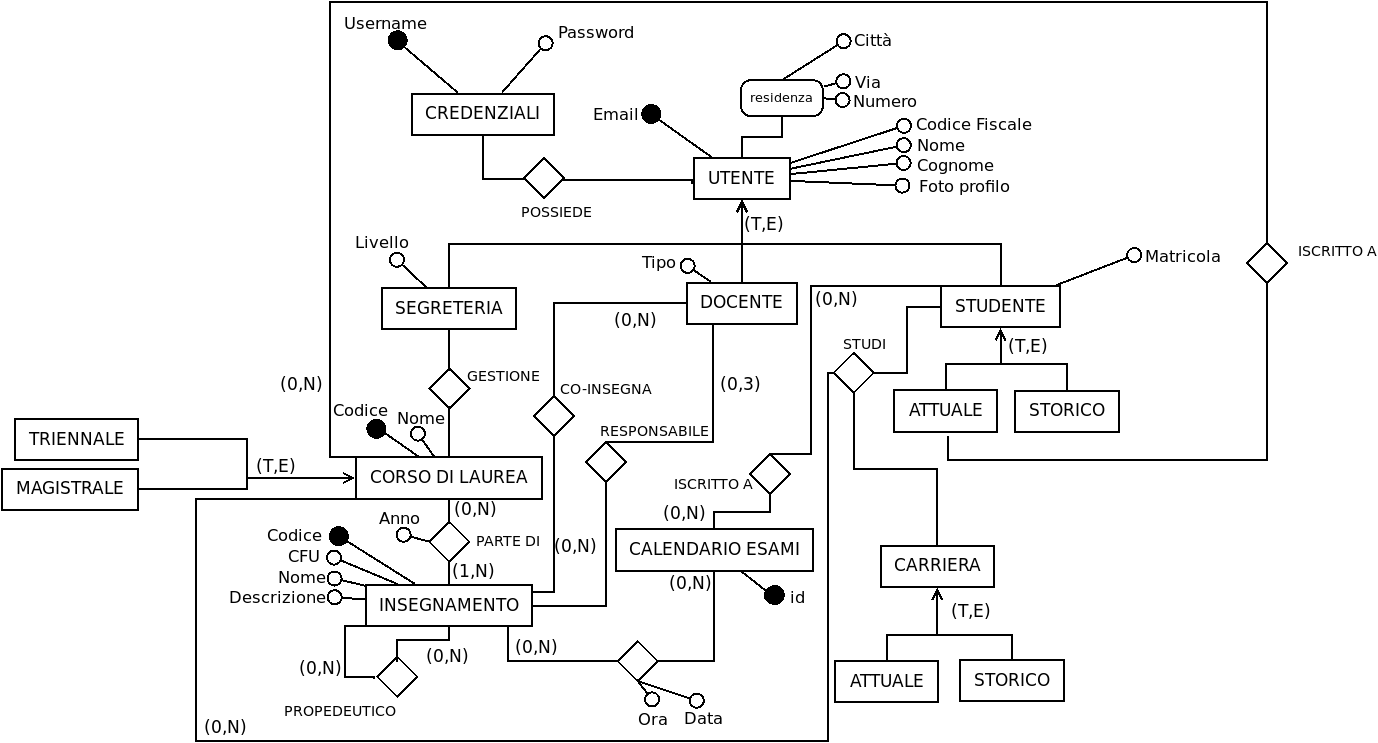
\includegraphics[scale=0.25]{images/SchemaER_PiGEU.png}

\section{Schema logico (relazionale) della base di dati}
Di seguito viene fornito lo schema logico della base di dati di PiGEU, tramite i comandi DDL utilizzati. Vengono fornite le tabelle del database in ordine alfabetico
\pagebreak

\lstset{
basicstyle=\footnotesize,
keywordstyle=\color{MidnightBlue}\bfseries,
identifierstyle=\color{Purple},
commentstyle=\color{Green}\itshape,
stringstyle=\color{Red}\ttfamily,
showstringspaces=false,
numbers=left, numberstyle=\tiny,
stepnumber=1, numbersep=5pt,
tabsize=4,
framexleftmargin=5mm, rulesepcolor=\color{LightGray},
frame=LtBr,
language={SQL}, ##
mathescape=true,
fontadjust=true,
breaklines=true,breakatwhitespace=true,breakautoindent
}


\begin{lstlisting}[
language={SQL},
title={Calendario Esami}]
CREATE TABLE public.calendario_esami (
    insegnamento character varying(10) NOT NULL,
    data date NOT NULL,
    ora time without time zone NOT NULL,
    id serial PRIMARY KEY,
    FOREIGN KEY (insegnamento) REFERENCES public.insegnamento(codice) ON UPDATE CASCADE ON DELETE CASCADE
);
\end{lstlisting}

\begin{lstlisting}[
language={SQL},
title={Carriera}]
CREATE TABLE public.carriera (
    studente character varying(50) NOT NULL,
    insegnamento character varying(10) NOT NULL,
    valutazione smallint,
    data date NOT NULL,
    PRIMARY KEY (studente, data, insegnamento),
    FOREIGN KEY (studente, insegnamento) REFERENCES public.insegnamenti_per_carriera(studente, insegnamento) ON UPDATE CASCADE ON DELETE CASCADE
);
\end{lstlisting}

\begin{lstlisting}[
language={SQL},
title={Carriera Storico}]
CREATE TABLE public.carriera_storico (
    studente character varying(50) NOT NULL,
    insegnamento character varying(10) NOT NULL,
    valutazione smallint,
    data date NOT NULL,
    PRIMARY KEY (studente, insegnamento, data),
    FOREIGN KEY (studente) REFERENCES public.studente_storico(utente) ON UPDATE CASCADE ON DELETE CASCADE
);
\end{lstlisting}

\begin{lstlisting}[
language={SQL},
title={Corso di Laurea}]
CREATE TABLE public.corso_di_laurea (
    codice character varying(5) NOT NULL,
    nome character varying(50),
    tipo character varying(50),
    PRIMARY KEY (codice)
);
\end{lstlisting}

\begin{lstlisting}[
language={SQL},
title={Credenziali}]
CREATE TABLE public.credenziali (
    username character varying(50) NOT NULL,
    password character varying(50),
    PRIMARY KEY (username),
    FOREIGN KEY (username) REFERENCES public.utente(email) ON UPDATE CASCADE ON DELETE CASCADE
);
\end{lstlisting}

\begin{lstlisting}[
language={SQL},
title={Docente}]
CREATE TABLE public.docente (
    utente character varying(50) NOT NULL,
    tipo character varying(50),
    PRIMARY KEY (utente)
);
\end{lstlisting}

\begin{lstlisting}[
language={SQL},
title={Docente Responsabile}]
CREATE TABLE public.docente_responsabile (
    docente character varying(50) NOT NULL,
    insegnamento character varying(10) NOT NULL
    PRIMARY KEY (docente, insegnamento),
    FOREIGN KEY (docente) REFERENCES public.docente(utente) ON UPDATE CASCADE ON DELETE CASCADE,
    FOREIGN KEY (insegnamento) REFERENCES public.insegnamento(codice) ON UPDATE CASCADE ON DELETE CASCADE
);
\end{lstlisting}

\begin{lstlisting}[
language={SQL},
title={Foto Profilo}]
CREATE TABLE public.foto_profilo (
    utente character varying(50) NOT NULL,
    path character varying(200),
    "timestamp" timestamp(6) without time zone NOT NULL,
    PRIMARY KEY (utente, "timestamp"),
    FOREIGN KEY (utente) REFERENCES public.utente(email) ON UPDATE CASCADE ON DELETE CASCADE
);
\end{lstlisting}

\begin{lstlisting}[
language={SQL},
title={Insegnamento}]
CREATE TABLE public.insegnamento (
    codice character varying(10) NOT NULL,
    nome character varying(50),
    descrizione text,
    cfu character(2),
    PRIMARY KEY (codice)
);
\end{lstlisting}

\begin{lstlisting}[
language={SQL},
title={Insegnamento parte di un Corso di Laurea}]
CREATE TABLE public.insegnamento_parte_di_cdl (
    insegnamento character varying(10) NOT NULL,
    corso_di_laurea character varying(5) NOT NULL,
    anno integer NOT NULL,
    PRIMARY KEY (insegnamento, corso_di_laurea, anno),
    FOREIGN KEY (corso_di_laurea) REFERENCES public.corso_di_laurea(codice) ON UPDATE CASCADE ON DELETE CASCADE,
    FOREIGN KEY (insegnamento) REFERENCES public.insegnamento(codice) ON UPDATE CASCADE ON DELETE CASCADE
);
\end{lstlisting}

\begin{lstlisting}[
language={SQL},
title={Utente}]
CREATE TABLE public.utente (
    email character varying(50) NOT NULL,
    nome character varying(50),
    cognome character varying(50),
    indirizzo character varying(255),
    citta character varying(255),
    codicefiscale character varying(16),
    emailpersonale character varying(60),
    PRIMARY KEY (email)
);
\end{lstlisting}

\begin{lstlisting}[
language={SQL},
title={Insegna}]
CREATE TABLE public.insegna (
    docente character varying(50) NOT NULL,
    insegnamento character varying(10) NOT NULL,
    PRIMARY KEY (docente, insegnamento),
    FOREIGN KEY (docente) REFERENCES public.docente(utente) ON UPDATE CASCADE ON DELETE CASCADE,
    FOREIGN KEY (insegnamento) REFERENCES public.insegnamento(codice) ON UPDATE CASCADE ON DELETE CASCADE,
    FOREIGN KEY (utente) REFERENCES public.utente(email) ON UPDATE CASCADE ON DELETE CASCADE
);
\end{lstlisting}

\begin{lstlisting}[
language={SQL},
title={Insegnamenti per carriera}]
CREATE TABLE public.insegnamenti_per_carriera (
    studente character varying(50) NOT NULL,
    insegnamento character varying(10) NOT NULL,
    "timestamp" timestamp(6) without time zone,
    PRIMARY KEY (studente, insegnamento),
    FOREIGN KEY (studente) REFERENCES public.studente(utente) ON UPDATE CASCADE ON DELETE CASCADE
);
\end{lstlisting}

\begin{lstlisting}[
language={SQL},
title={Iscrizione}]
CREATE TABLE public.iscrizione (
    studente character varying(50) NOT NULL,
    esame integer NOT NULL,
    PRIMARY KEY (studente, esame),
    FOREIGN KEY (studente) REFERENCES public.studente(utente) ON UPDATE CASCADE ON DELETE CASCADE
);
\end{lstlisting}

\begin{lstlisting}[
language={SQL},
title={Propedeuticità}]
CREATE TABLE public.propedeuticita (
    insegnamento1 character varying(10) NOT NULL,
    insegnamento2 character varying(10) NOT NULL,
    corso_di_laurea character varying(5) NOT NULL,
    PRIMARY KEY (insegnamento1, insegnamento2, corso_di_laurea),
    FOREIGN KEY (insegnamento1) REFERENCES public.insegnamento(codice) ON UPDATE CASCADE ON DELETE CASCADE,
    FOREIGN KEY (insegnamento2) REFERENCES public.insegnamento(codice) ON UPDATE CASCADE ON DELETE CASCADE
    FOREIGN KEY (corso_di_laurea) REFERENCES public.corso_di_laurea(codice) ON UPDATE CASCADE ON DELETE CASCADE
);
\end{lstlisting}

\begin{lstlisting}[
language={SQL},
title={Segreteria}]
CREATE TABLE public.segreteria (
    utente character varying(50) NOT NULL,
    livello character varying(9) NOT NULL,
    PRIMARY KEY (utente),
    FOREIGN KEY (utente) REFERENCES public.utente(email) ON UPDATE CASCADE ON DELETE CASCADE
);
\end{lstlisting}

\begin{lstlisting}[
language={SQL},
title={Studente}]
CREATE TABLE public.studente (
    utente character varying(50) NOT NULL,
    matricola serial NOT NULL,
    corso_di_laurea character varying(5),
    PRIMARY KEY (utente),
    FOREIGN KEY (corso_di_laurea) REFERENCES public.corso_di_laurea(codice) ON UPDATE CASCADE ON DELETE CASCADE,
    FOREIGN KEY (utente) REFERENCES public.utente(email) ON UPDATE CASCADE ON DELETE CASCADE
);

\end{lstlisting}

\begin{lstlisting}[
language={SQL},
title={Studente Storico}]
CREATE TABLE public.studente_storico (
    utente character varying(50) NOT NULL,
    matricola integer,
    corso_di_laurea character varying(5),
    PRIMARY KEY (utente),
    FOREIGN KEY (utente) REFERENCES public.utente_storico(email) ON UPDATE CASCADE ON DELETE CASCADE
);
\end{lstlisting}

\begin{lstlisting}[
language={SQL},
title={Utente Storico}]
CREATE TABLE public.utente_storico (
    email character varying(50) NOT NULL,
    nome character varying(50),
    cognome character varying(50),
    indirizzo character varying(255),
    citta character varying(255),
    codicefiscale character varying(16),
    emailpersonale character varying(60),
    PRIMARY KEY (email)
);
\end{lstlisting}

















\subsection{Si enuncino i tre teoremi dei triangoli rettangoli, riportando enunciato e figure per spiegare meglio} \hspace{50} p872
\subsection{Si enunci il teorema della corda}
\subsection{Definire cosa sia:}
a. Una funzione: \\\\\\\\
b. Il Dominio e il Codominio di funzione: \\\\\\\\
c. una funzione Dispari con relativo esempio convincente : \\\\\\\\\\\\
d. Una funzione invertibile: spiegare bene nel dettaglio: \\\\\\\\\\\\\\
e. Lo zero di una funzione, spiegazione con anche grafico di esempio: \\\\\\\\\\
f. Il teorema di Bayes: enunciarlo con la formula e dire le analogie e differenze con il teorema della probabilità condizionata  (valuta la possibilità di esporre allora anche il teorema della probabilità condizionata) \\\\\\\\\\\\\\\\\\\\\\\\\\\\\\\\\\\\\\\\\\\\\\\\\\

\section{Esercizi pratici}
\subsection{Si risolvano i seguenti esercizi}


\title{Il mio primo documento LaTeX}
\author{Nome dell'autore}
\date{}




Questo è un paragrafo di testo. In LaTeX, i paragrafi vengono separati da una o più righe vuote.

È possibile scrivere testo in \textbf{grassetto} o \emph{corsivo}.

\section{Una sezione}

Questo è un paragrafo nella sezione \emph{Una sezione}.

\subsection{Una sottosezione}

Questo è un paragrafo nella sottosezione \emph{Una sottosezione}.

\subsubsection{Una sottosottosezione}

Questo è un paragrafo nella sottosottosezione \emph{Una sottosottosezione}.





\end{document}